\documentclass{article}

% packages and stuff
\usepackage[utf8]{inputenc}
\usepackage[headheight = 18pt, footskip = 10pt]{geometry}
    \geometry{a4paper}
    \geometry{left=0.5in, right=0.5in, top=.95in, bottom=.95in}
\usepackage{graphicx}
\usepackage{amsmath}
%Better boxed command in math mode
\usepackage{empheq}
%Input text files and code
\usepackage{verbatim}
%Bold math
\usepackage{bm}
%Cancel to in math mode
\usepackage{cancel}
% Input standalone tex documents
\usepackage{standalone}
\usepackage{subcaption}
\usepackage{ulem}
\usepackage{bigstrut}
\usepackage{bm}
\usepackage{multirow}
\usepackage{calc}
\usepackage{xkeyval}
\usepackage{color, soul}
\usepackage{ifthen}
\usepackage{import}
\usepackage{times}
\usepackage{longtable}
\usepackage{tabularx}
\usepackage{multicol}
\usepackage{wrapfig}
\usepackage[font={small,it}]{caption}
\usepackage[version=4]{mhchem}
\usepackage{booktabs}
\usepackage{longtable}
\usepackage{epigraph}

%New colors defined below
\definecolor{codegreen}{rgb}{0,0.6,0}
\definecolor{codegray}{rgb}{0.5,0.5,0.5}
\definecolor{codepurple}{rgb}{0.58,0,0.82}
\definecolor{backcolour}{rgb}{0.95,0.95,0.92}

% Include external pdf documents
\usepackage{pdfpages}

%Nice captions in floating figures
\usepackage{caption}

%%%%%%%%%%%%%%%%%%%%%%%%%%%%%%%%%%%%%%%%%%%%%%%%%%%%%%%%%%%%%%%%%%%%%%%%%%%%%%%%
\usepackage{fancyvrb}
\usepackage{comment}
\usepackage{enumerate}
\usepackage{subfiles}

%%%%%%%%%%%%%%%%%%%%%%%%%%%%%%%%%%%%%%%%%%%%%%%%%%%%%%%%%%%%%%%%%%%%%%%%%%%%%%%

% capital H is a champion
\usepackage{float}
    \restylefloat{table}

% make section styles non-lame
\usepackage{sectsty}
    \allsectionsfont{\mdseries\upshape}

% easy coloring for todo notes
\newcommand{\done}{\todo[inline, color=green]{(DONE)}{}}
\newcommand{\notdone}{\todo[inline, color=red]{(NOT DONE)}{}}
\newcommand{\fix}[1]{\todo[inline, color=red!75]{(FIX) #1}{}}
\newcommand{\discuss}[1]{\todo[inline, color=blue!40]{(DISCUSS) #1}{}}
\newcommand{\note}[1]{\todo[inline, color=yellow!20]{(NOTE) #1}}
\newcommand{\review}{\todo[inline, color=red!45!yellow!45]{(REVIEW)}{}}


\pagenumbering{gobble}
\setlength\parindent{10pt}
\setlength{\parskip}{0pt}
\setlength{\abovedisplayskip}{0pt}
\setlength{\belowdisplayskip}{0pt}
\relpenalty=10000 % don't split equations!!
\binoppenalty=10000 % don't split equations!!

\newcommand{\FigSiz}{0.37\textwidth}

% Set global figure size variable

\makeatletter
\define@key{Gin}{figsize}[true]{%
    \edef\@tempa{{Gin}{width=\FigSiz}}%
    \expandafter\setkeys\@tempa
}
\makeatother


%%%%%%%%%%%%%%%%%%%%%%%%%%%%%%%%%%%%%%%%%%%%%%%%%%%%%%%%%%%%%%%%%%%%%%%%%%%%%%%%%%%%%%%%%%%%%%%


% Custom title
\pagenumbering{arabic}
\usepackage{lastpage}
\usepackage{fancyhdr}
    \fancyhead{}
    \fancyfoot{}
    \pagestyle{fancy}
    \chead{\Large CS575: Project 5}
    \lhead{\Large Andrew Alferman}
    \rhead{\Large \today}
    \cfoot{\thepage  ~\ of ~\pageref{LastPage}}

\usepackage{titlesec}
\titlespacing*{\subsection}
{0pt}{0.65\baselineskip}{0.65\baselineskip}

%%%%%%%%%%%%%%%%%%%%%%%%%%%%%%%%%%%%%%%%%%%%%%%%%%%%%%%%%%%%%%%%%%%%%%%%%%%%%%%%%%%%%%%%%%%%%%%
\begin{document}



% Brief summary of the assignment
The purpose of this assignment was to test and demonstrate the relative speeds of array multiplication and array multiplication-reduction using both non-SIMD (single instruction multiple data) and SIMD code.

\subsection*{Question 1}
\textit{What machine did you run the experiment on?}

The experiment was run on flip at a time when the load average was approximately 0.35.

\subsection*{Question 2}
\textit{Show a table and graph of the array multiplication timing experiment.}

Graphs of the computation speed and the SSE/non-SSE speedup are found in Figures \ref{fig:Speed} and \ref{fig:Speedup}, respectively.  A table of the values used to generate these graphs can be found in Table \ref{tab:Data} of Appendix \ref{app:Data}.

\begin{figure}[h]
	\centering
        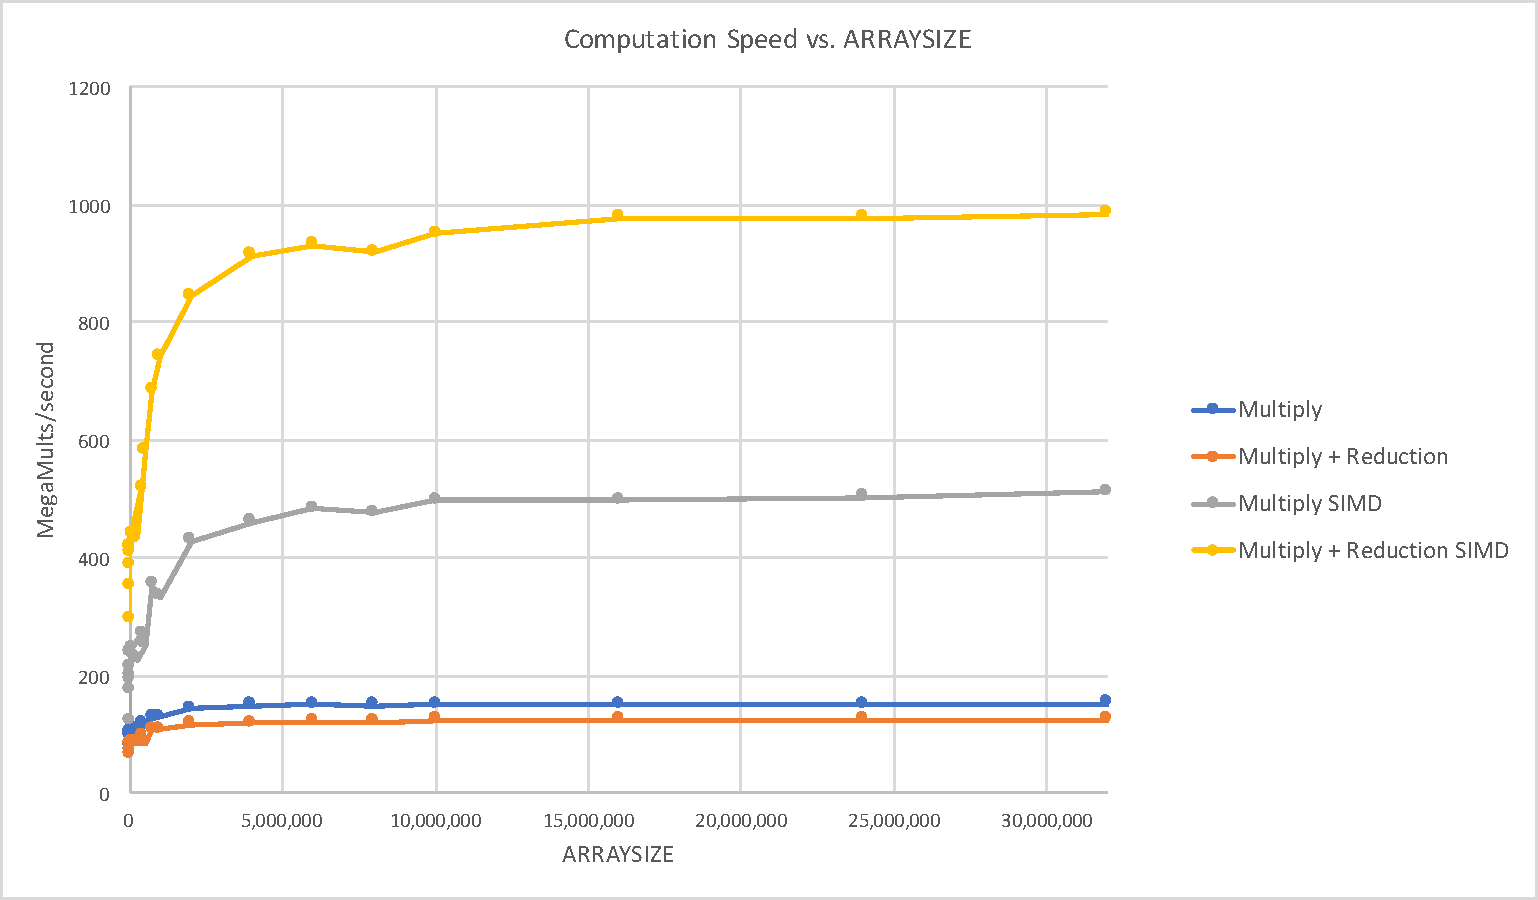
\includegraphics[width=0.7\linewidth]{Speeds.pdf}
        \caption{Speed of the experiment.}
        \label{fig:Speed}
\end{figure}

\begin{figure}[h]
	\centering
        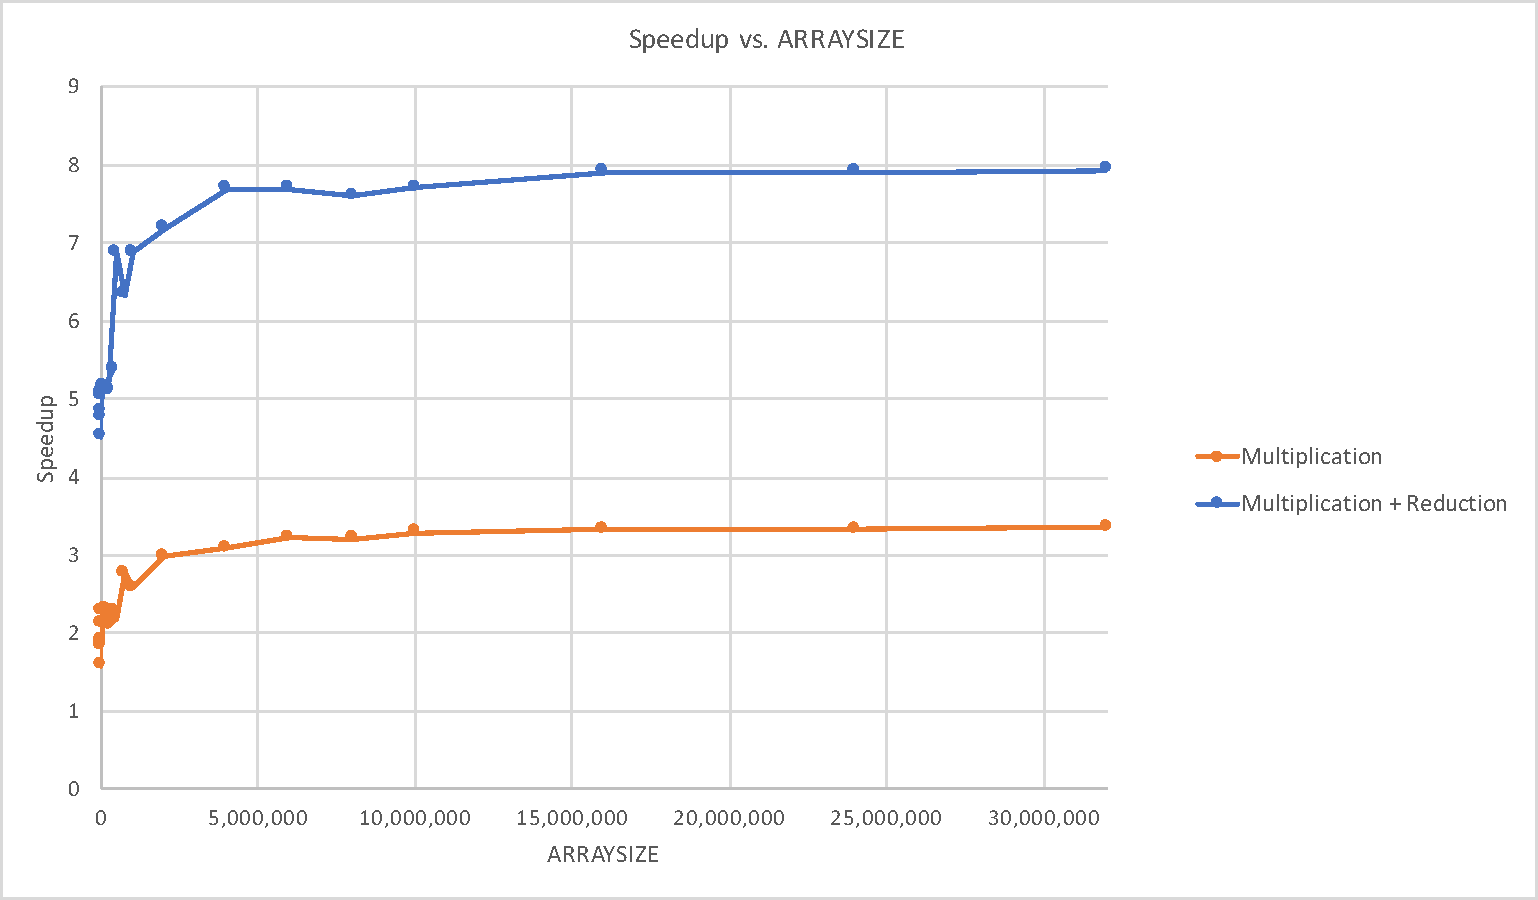
\includegraphics[width=0.7\linewidth]{Speedup.pdf}
        \caption{SIMD Speedups.}
        \label{fig:Speedup}
\end{figure}

\newpage
\subsection*{Question 3}
\textit{What patterns are you seeing in the speedups?}

Without SIMD SSE, multiplication with reduction is slightly slower than multiplication, although the difference in speed is relatively small.  With SIMD SSE, multiplication with reduction is substantially faster than multiplication alone.  Both multiplication and multiplication with reduction are much faster when using SIMD SSE.

The speedup of multiplication with reduction was more than twice the speedup of multiplication alone.

\subsection*{Question 4}
\textit{Are the speedups consistent across a variety of array sizes?}

Both the speeds and the speedups were smaller when using very small array sizes.  However, after reaching an array size of approximately 2 million or greater, the speeds and speedups remained very consistent up through the largest array size tested (32 million).

\subsection*{Question 5}
\textit{Why or why not are the speedups consistent across a variety of array sizes?}

The speedups are largely consistent because this experiment may be parallelized/vectorized very easily.  All of the computations involve multiplication or addition of values in an array, which requires few serial operations.  Additionally, the array sizes used were generally very large, which further drives up the parallel fraction and allows the speedup to approach the number of floats computed at-a-time.  This is similar to Ahmdal's law, however the parallelization occurs in a single core executing multiple instructions simultaneously, therefore the number of parallel instructions is analogous to the number of cores used in a multiprocessing experiment.  Furthermore, assembly language was used for the SSE SIMD, which minimizes the amount of work that must be accomplished to set up the parallelism/vectorization.

\subsection*{Question 6}
\textit{Knowing that SSE SIMD is 4-floats-at-a-time, why could you get a speedup of $<$ 4.0 or $>$ 4.0 in the array multiplication?}

The speedup for the array multiplication is less than 4.0 because there is a small overhead cost in setting up the computation.  This prevents the experiment from running with 100\% efficiency, and thus the speedup is less than the number of floats computed at-a-time.

\subsection*{Question 7}
\textit{Knowing that SSE SIMD is 4-floats-at-a-time, why could you get a speedup of $<$ 4.0 or $>$ 4.0 in the array multiplication-reduction?}

The speedup for the array multiplication-reduction is greater than 4.0 when using SSE SIMD with 4-floats-at-a-time because the assembly code writes to the registers instead of constantly having to work with the stack.  In contrast, the non-SSE SIMD code has to conduct two separate operations using the stack.  Additionally, there are few additional instructions in assembly language at each iteration with multiplication-reduction versus multiplication alone.  Because of this, the speedup approaches double the number of floats-at-a-time, which is evidenced by a speedup in Figure \ref{fig:Speedup} of slightly less than 8.0 with multiplication-reduction.

\newpage
\section{Appendices}
\subsection{Tables of Generated Data}
\label{app:Data}


\begin{longtable}{|l|l|l|}
\caption{Raw Data Generated}\label{tab:Data}\\
\hline
Run               & ARRAYSIZE & MegaMults \\ \hline
Mult Non-SIMD     & 1000      & 77.51     \\ \hline
Mult Non-SIMD     & 2000      & 96.20     \\ \hline
Mult Non-SIMD     & 4000      & 104.91    \\ \hline
Mult Non-SIMD     & 8000      & 101.66    \\ \hline
Mult Non-SIMD     & 10000     & 101.59    \\ \hline
Mult Non-SIMD     & 20000     & 104.46    \\ \hline
Mult Non-SIMD     & 400000    & 117.79    \\ \hline
Mult Non-SIMD     & 80000     & 106.85    \\ \hline
Mult Non-SIMD     & 160000    & 100.24    \\ \hline
Mult Non-SIMD     & 250000    & 108.43    \\ \hline
Mult Non-SIMD     & 500000    & 115.46    \\ \hline
Mult Non-SIMD     & 750000    & 127.81    \\ \hline
Mult Non-SIMD     & 1000000   & 129.26    \\ \hline
Mult Non-SIMD     & 2000000   & 143.69    \\ \hline
Mult Non-SIMD     & 4000000   & 148.51    \\ \hline
Mult Non-SIMD     & 6000000   & 149.92    \\ \hline
Mult Non-SIMD     & 8000000   & 148.87    \\ \hline
Mult Non-SIMD     & 10000000  & 151.36    \\ \hline
Mult Non-SIMD     & 16000000  & 149.78    \\ \hline
Mult Non-SIMD     & 24000000  & 151.39    \\ \hline
Mult Non-SIMD     & 32000000  & 152.22    \\ \hline
Mult-sum Non-SIMD & 1000      & 65.12     \\ \hline
Mult-sum Non-SIMD & 2000      & 72.38     \\ \hline
Mult-sum Non-SIMD & 4000      & 81.26     \\ \hline
Mult-sum Non-SIMD & 8000      & 81.22     \\ \hline
Mult-sum Non-SIMD & 10000     & 83.32     \\ \hline
Mult-sum Non-SIMD & 20000     & 81.52     \\ \hline
Mult-sum Non-SIMD & 400000    & 96.62     \\ \hline
Mult-sum Non-SIMD & 80000     & 85.46     \\ \hline
Mult-sum Non-SIMD & 160000    & 84.47     \\ \hline
Mult-sum Non-SIMD & 250000    & 85.56     \\ \hline
Mult-sum Non-SIMD & 500000    & 84.56     \\ \hline
Mult-sum Non-SIMD & 750000    & 107.89    \\ \hline
Mult-sum Non-SIMD & 1000000   & 107.76    \\ \hline
Mult-sum Non-SIMD & 2000000   & 117.66    \\ \hline
Mult-sum Non-SIMD & 4000000   & 118.62    \\ \hline
Mult-sum Non-SIMD & 6000000   & 121.19    \\ \hline
Mult-sum Non-SIMD & 8000000   & 120.90    \\ \hline
Mult-sum Non-SIMD & 10000000  & 123.32    \\ \hline
Mult-sum Non-SIMD & 16000000  & 123.44    \\ \hline
Mult-sum Non-SIMD & 24000000  & 123.64    \\ \hline
Mult-sum Non-SIMD & 32000000  & 124.08    \\ \hline
Mult SIMD         & 1000      & 122.58    \\ \hline
Mult SIMD         & 2000      & 175.32    \\ \hline
Mult SIMD         & 4000      & 200.85    \\ \hline
Mult SIMD         & 8000      & 191.92    \\ \hline
Mult SIMD         & 10000     & 214.29    \\ \hline
Mult SIMD         & 20000     & 238.24    \\ \hline
Mult SIMD         & 400000    & 269.93    \\ \hline
Mult SIMD         & 80000     & 244.33    \\ \hline
Mult SIMD         & 160000    & 231.55    \\ \hline
Mult SIMD         & 250000    & 227.45    \\ \hline
Mult SIMD         & 500000    & 252.16    \\ \hline
Mult SIMD         & 750000    & 353.17    \\ \hline
Mult SIMD         & 1000000   & 333.55    \\ \hline
Mult SIMD         & 2000000   & 428.71    \\ \hline
Mult SIMD         & 4000000   & 459.24    \\ \hline
Mult SIMD         & 6000000   & 483.53    \\ \hline
Mult SIMD         & 8000000   & 476.70    \\ \hline
Mult SIMD         & 10000000  & 497.60    \\ \hline
Mult SIMD         & 16000000  & 497.27    \\ \hline
Mult SIMD         & 24000000  & 503.03    \\ \hline
Mult SIMD         & 32000000  & 510.58    \\ \hline
Mult-sum SIMD     & 1000      & 293.85    \\ \hline
Mult-sum SIMD     & 2000      & 349.71    \\ \hline
Mult-sum SIMD     & 4000      & 386.88    \\ \hline
Mult-sum SIMD     & 8000      & 409.48    \\ \hline
Mult-sum SIMD     & 10000     & 418.57    \\ \hline
Mult-sum SIMD     & 20000     & 413.81    \\ \hline
Mult-sum SIMD     & 400000    & 518.89    \\ \hline
Mult-sum SIMD     & 80000     & 439.98    \\ \hline
Mult-sum SIMD     & 160000    & 431.31    \\ \hline
Mult-sum SIMD     & 250000    & 435.96    \\ \hline
Mult-sum SIMD     & 500000    & 581.53    \\ \hline
Mult-sum SIMD     & 750000    & 682.09    \\ \hline
Mult-sum SIMD     & 1000000   & 740.52    \\ \hline
Mult-sum SIMD     & 2000000   & 844.68    \\ \hline
Mult-sum SIMD     & 4000000   & 912.21    \\ \hline
Mult-sum SIMD     & 6000000   & 931.01    \\ \hline
Mult-sum SIMD     & 8000000   & 917.73    \\ \hline
Mult-sum SIMD     & 10000000  & 949.49    \\ \hline
Mult-sum SIMD     & 16000000  & 975.98    \\ \hline
Mult-sum SIMD     & 24000000  & 976.62    \\ \hline
Mult-sum SIMD     & 32000000  & 984.21    \\ \hline
\end{longtable}

\end{document}
